\documentclass[11pt]{article}
\usepackage[spanish]{babel}
\usepackage{natbib}
\usepackage{url}
\usepackage[utf8x]{inputenc}
\usepackage{amsmath}
\usepackage{amssymb}
\usepackage{graphicx}
\graphicspath{{images/}}
\usepackage{parskip}
\usepackage{fancyhdr}
\usepackage{vmargin}
\usepackage{apalike}
%\usepackage{hyperref}
%\hypersetup{
%    colorlinks=true,
%    linkcolor=blue,
%    filecolor=magenta,      
%    urlcolor=cyan,
%}

\setmarginsrb{3 cm}{2.5 cm}{3 cm}{2.5 cm}{1 cm}{1.5 cm}{1cm}{1.5 cm}

\title{Proyectos}						% Title
\author{J. Eduardo Sánchez Posadas}					%Author
\date{\today}											% Date

\makeatletter
\let\thetitle\@title
\let\theauthor\@author
\let\thedate\@date
\makeatother

\pagestyle{fancy}
\fancyhf{}
\rhead{GUI con Java}
\lhead{\thetitle}
\rfoot{\thepage}
\lfoot{FES Aragón - UNAM}

\begin{document}

%%%%%%%%%%%%%%%%%%%%%%%%%%%%%%%%%%%%%%%%%%%%%%%%%%%%%%%%%%%%%%%%%%%

\begin{titlepage}
	\centering
    \vspace*{0.5 cm}

\includegraphics[scale=0.05]{pics/escudo.png} \\[1.0 cm] 
%University Logo
\textsc{\Large Universidad Nacional Autónoma de México}\\[2.0 cm]
% University Name
\textsc{\Large FES Aragón\\ Ingeniería en Computación}\\[0.5 cm]
% Course Code
\textsc{\large Interfaces Gráficas de Usuario \\ con Java}\\[0.5
cm] % Course Name
	\rule{\linewidth}{0.2 mm} \\[0.4 cm]
	{ \huge \bfseries \thetitle}\\
	\rule{\linewidth}{0.2 mm} \\[1.5 cm]
	 			{Autor: \large \theauthor}
% 	\begin{minipage}{0.4\textwidth}
% 		\begin{flushleft} \large
% 			\emph{Nombre: Nombre(s) Apellido(s]}\\
%
% 			\end{flushleft}
% 			\end{minipage}~
% 			\begin{minipage}{0.4\textwidth}
% 			\begin{flushright} \large
% 			\emph{Número de Cuenta} \\
% 											% Your Student Number
% 		\end{flushright}
% 	\end{minipage}\\[2 cm]
	
	{\large \thedate}\\[2 cm]
 
	\vfill
	
\end{titlepage}

%%%%%%%%%%%%%%%%%%%%%%%%%%%%%%%%%%%%%%%%%%%%%%%%%%%%%%%%%%%%%%%%%%%

\tableofcontents
\pagebreak

%%%%%%%%%%%%%%%%%%%%%%%%%%%%%%%%%%%%%%%%%%%%%%%%%%%%%%%%%%%%%%%%%%%

\section{Fechas importantes}
\begin{center}
\begin{table}[h]
\begin{tabular}{|c|c|c|}
\hline
\textbf{Fecha} & \textbf{Evento}       & \textbf{Descripción}                                                                                                                                                                                                                                                                                                            \\ \hline
7 de Julio     & Elección del proyecto & \begin{tabular}[c]{@{}c@{}}Deberán elegir el proyecto a realizar, un representante\\ del equipo deberá enviar un correo con los nombres y \\ correos de los integrantes y el proyecto que\\ decidieron realizar. Posteriormente se enivará\\ a cada uno el acceso la carpeta de Drive\\ donde subirán su proyecto.\end{tabular} \\ \hline
14 de Julio    & Primer avance         & \begin{tabular}[c]{@{}c@{}}Se deberá subir el código fuente del proyecto a\\ su carpeta en Drive y en un documento de word\\ cada integrante del equipo escribirá las dudas o\\ problemas que tienen hasta este día y posteriormente\\ se enviarán los comentarios al respecto.\end{tabular}                                    \\ \hline
18 de Julio    & Segundo avance        & \begin{tabular}[c]{@{}c@{}}Se deberá subir el código fuente del proyecto a\\ su carpeta en Drive y en un documento de word\\ cada integrante del equipo escribirá las dudas o\\ problemas que tienen hasta este día y posteriormente\\ se enviarán los comentarios al respecto.\end{tabular}                                    \\ \hline
22 de Julio    & Entrega               & \begin{tabular}[c]{@{}c@{}}Se deberá subir su carpeta de Drive el ejecutable del\\ proyecto, además del código fuente.\end{tabular}                                                                                                                                                                                             \\ \hline
25 de Julio    & Calificación Final    & \begin{tabular}[c]{@{}c@{}}Se subirá la calificación del proyecto en la plataforma\\ del CAE a las 15:00\end{tabular}                                                                                                                                                                                                           \\ \hline
\end{tabular}
\end{table}
\end{center}

\section{Aspectos a evaluar}
\begin{center}
\begin{tabular}{|c||c|}
\hline 
\rule[-1ex]{0pt}{2.5ex} Rubro & Porcentaje \\ 
\hline \hline
\rule[-1ex]{0pt}{2.5ex} Funcionalidad & 50\% \\ 
\hline 
\rule[-1ex]{0pt}{2.5ex} Uso de componentes & 25\% \\ 
\hline 
\rule[-1ex]{0pt}{2.5ex} Uso de contenedores & 25\% \\ 
\hline 
\rule[-1ex]{0pt}{2.5ex} Uso de cuadros de diálogo & +10\% \\ 
\hline 
\rule[-1ex]{0pt}{2.5ex} Estética de la interfaz & +15\% \\ 
\hline 
\rule[-1ex]{0pt}{2.5ex} Total & $\pm$ 125\% \\ 
\hline 
\end{tabular} 
\end{center}


\section{Generador de Funciones Sinusoidales}
\subsection{Introducción}

Un \emph{generador de señales}, de \emph{funciones} o de
\emph{formas de onda} es un dispositivo electrónico de
laboratorio que genera patrones de señales periódicas o no
periódicas tanto analógicas como digitales. Se emplea
normalmente en el diseño, prueba y reparación de dispositivos
electrónicos; aunque también puede tener usos artísticos.

Hay diferentes tipos de generadores de señales según el
propósito y aplicación que corresponderá con el precio.
Tradicionalmente los generadores de señales eran dispositivos
estáticos apenas configurables, pero actualmente permiten la
conexión y control desde un PC. Con lo que pueden ser
controlados mediante software hecho a medida según la
aplicación, aumentando la flexibilidad. \citep{gdf}

\subsection{Señal}
\textbf{Señal}: se define como una magnitud física o detectable
mediante la que se puede transmitir mensajes o información.
Matemáticamente una señal es una función de una variable
independiente. Ejemplo:
$$x(t) = 3\sin(2t)$$
En el ejemplo anterior $t$ es la variable independiente.
Ejemplos en la realidad:
\begin{itemize}
\item Señales de audio de micrófono
\item Voltaje o intensidad en un circuito
\item Flujo de bits en proporcionados por un ordenador
\citep{iss}
\end{itemize}

\begin{figure}[h]
\centering
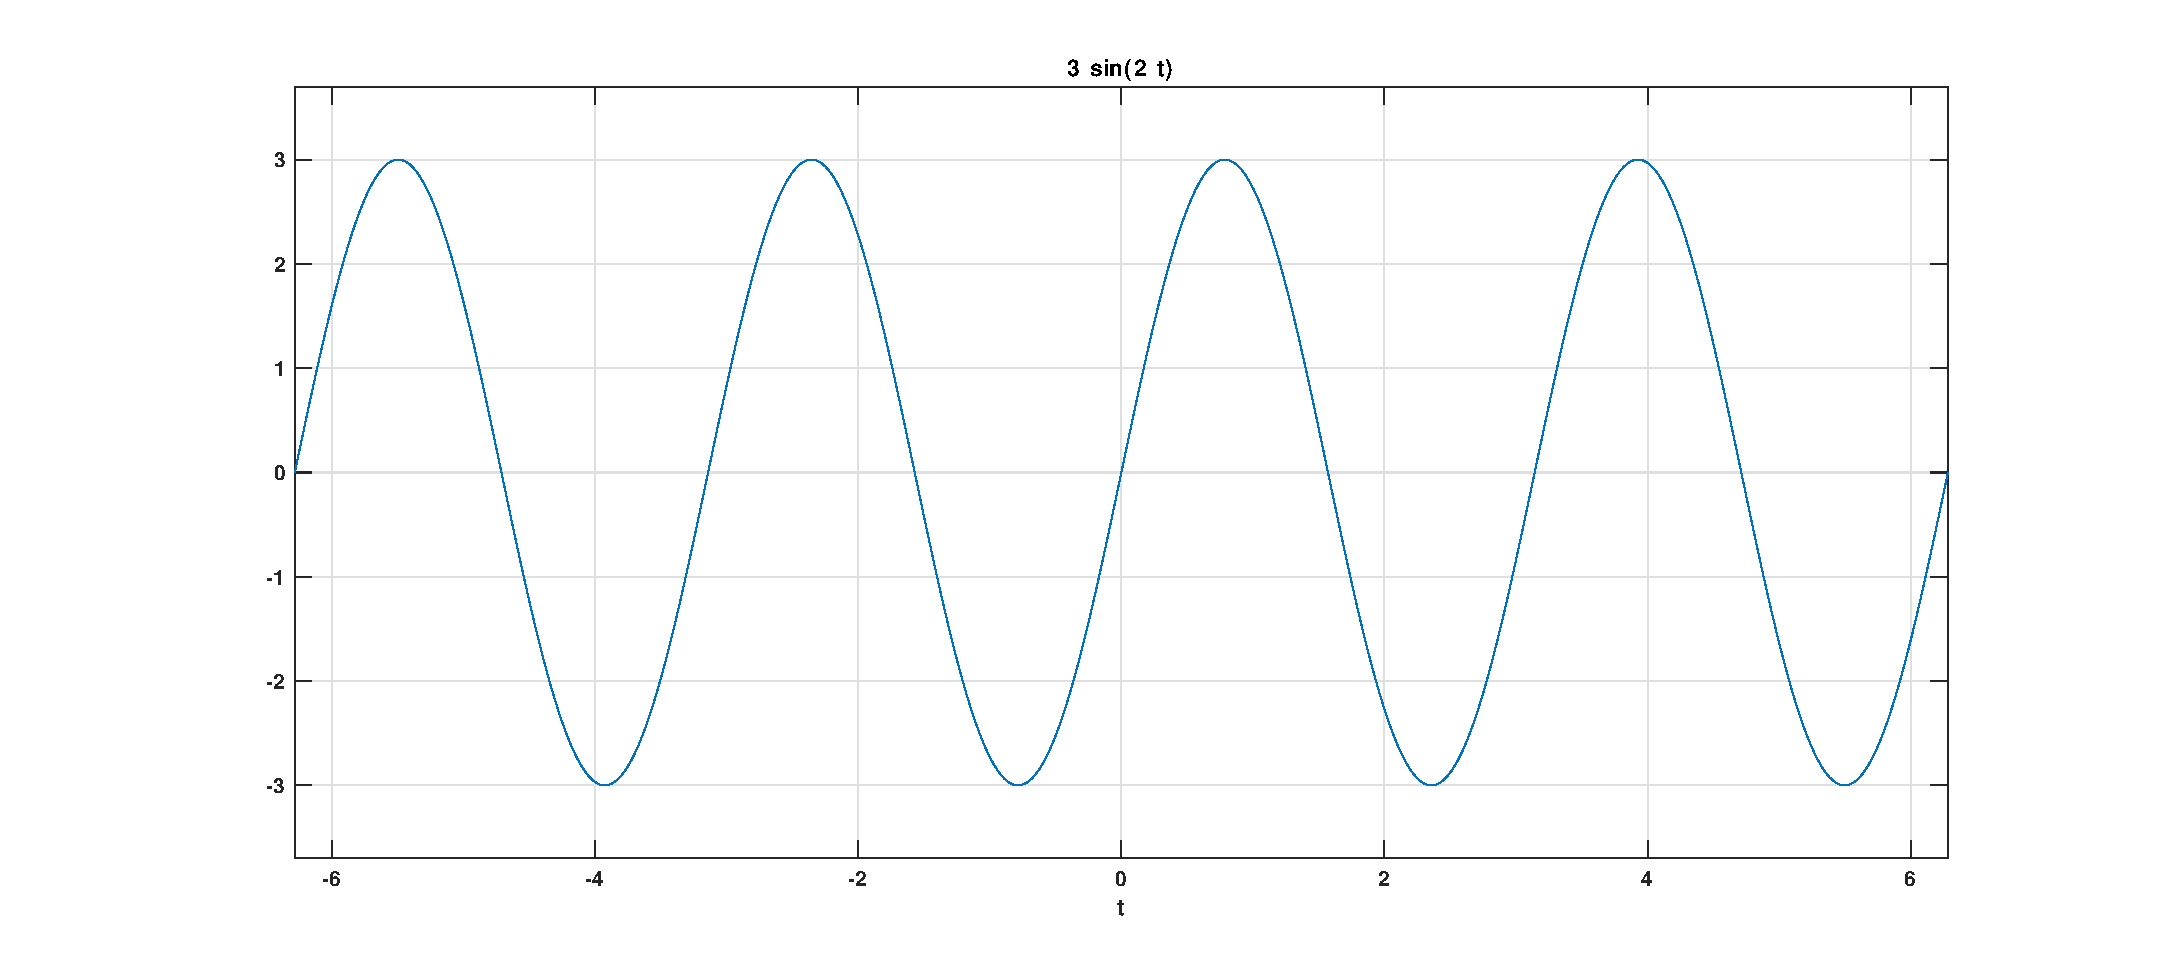
\includegraphics[scale=0.3]{pics/3sin2t.eps} 
\caption{Señal $3\sin(2t)$}
\end{figure}
\newpage
Una señal sinusoidal puede ser descrita por las siguientes
expresiones matemáticas:

$$y(x)=A \sin(\omega x + \phi)$$
$$y(x)=A \sin(2\pi ft + \phi)$$
$$y(x)=A \sin \left(\frac{2\pi}{T}x+\phi\right)$$
donde:\\
\begin{itemize}
\item $A$ es la amplitud de oscilación.
\item $\omega$ es la velocidad angular; $\omega=2\pi f$
\item $f$ es la frecuencia de oscilación.
\item $T$ es el periodo de oscilación; $T=1/f$
\item $\omega x + \phi$ es la fase de oscilación.
\item $\phi$ es la fase inicial.
\end{itemize}

\begin{figure}
\centering
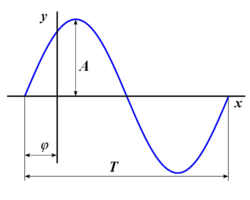
\includegraphics[scale=0.7]{pics/sin_c.png} 
\caption{Características de una señal sinusoidal}
\end{figure}

\subsection{Requerimientos}
Debe realizar una aplicación en Java con interfaz gráfica donde
se pueda graficar señales sinusoidal y cosenoidal. Debe tener
mínimo lo siguiente:

\begin{itemize}
\item Elegir entre sinusoidal y cosenoidal
\item Modificar amplitud
\item Modificar frecuencia
\item Modificar el \emph{offset}\footnote{Es el desplazamiento
vertical de la señal}
\item Lista de las señales generadas
\item Añadir mas de una señal
\item Editar una señal
\item Eliminar una señal
\item Modificar el color de la señal
\item Mostrar valor pico-pico
\item Mostrar valor $RMS$ de la señal
\item Guardar una imagen en JPEG o PNG
\item Malla
\item Cada componente deberá tener \textsf{toolTipText} explicando brevemente que función realiza. 
\end{itemize}

En la Figura 3 se sugiere la interfaz gráfica\footnote{Código disponible aquí: }
%\href{http://www.sharelatex.com}{repositorio en GitHub} 

\begin{figure}[h]
\centering
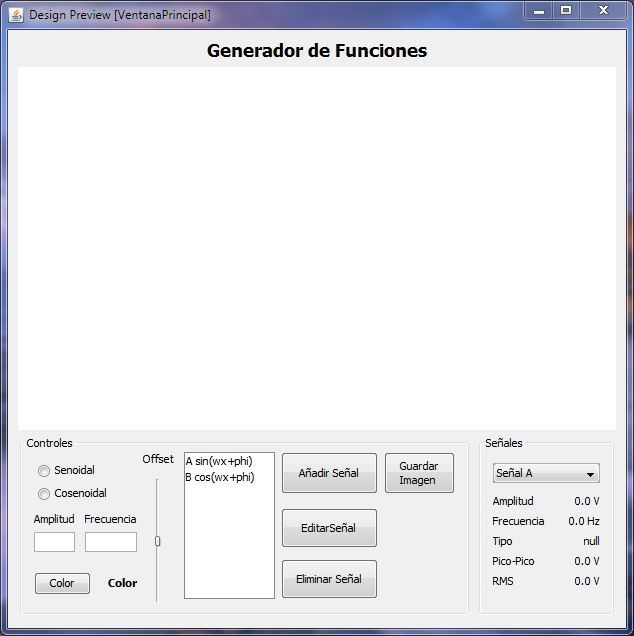
\includegraphics[scale=0.5]{pics/img_1.JPG} 
\caption{Sugerencia de interfaz gráfica para este proyecto.}
\end{figure}



\section{Sistema de Votación}
\subsection{Descripción}
Voto electrónico es una expresión que comprende varios tipos de votación, que abarca tanto modos electrónicos de emitir votos (voto por internet) como medios electrónicos de contar los votos.

Las tecnologías para el voto electrónico pueden incluir tarjetas perforadas, sistemas de votación mediante escáneres ópticos y quioscos de votación especializados (incluso sistemas de votación autocontenidos sistemas de votación de Registro o Grabación Electrónica Directa, DRE por sus siglas en inglés). También puede referirse a la transmisión de papeletas y votos por vía telefónica, redes de computación privadas o por Internet.

Las tecnologías del voto electrónico pueden acelerar el conteo de los votos y proveer una mejor accesibilidad para los votantes con algún tipo de discapacidad. Sin embargo, ha sido calificado como anticonstitucional en algunos países (como Alemania1) con el argumento de "no permitir la fiscalización del proceso" por personas sin conocimientos altamente especializados.

No se ha encontrado un modelo formal (conocido en la jerga como \textit{Model checking}) que garantice la seguridad de un sistema electrónico de votación. Los modelos formales son un requisito básico para mostrar que un sistema no tiene fallas triviales.

\subsection{Requerimientos}

Para este proyecto se requerirá lo siguiente:
\begin{itemize}
\item Ventana para registro de candidatura, y que lo guarde en archivo serializable \texttt{.cnd}:
\begin{itemize}
\item Partido o independiente
\item Color de partido o color de independiente
\item Logo de partido o independiente
\item Nombre del propietario
\item Nombre del suplente
\end{itemize}
\item Ventana para registro de electores, y que lo guarde en archivo serializable \texttt{.vota}:
\begin{itemize}
\item Nombre
\item Identificador (Clave de Elector o Matricula)
\end{itemize}
\item En el sistema se debe poder registrar a $n$ cantidad de candidatos y $m$ cantidad de electores.
\item Ventana de votación.
\item  Se debe establecer una hora de inicio y fin de la jornada electoral. Debe estar visible un reloj con segundos junto con la hora de inicio y la hora de fin en la ventana de votación. Una vez finalizado el tiempo ningún votante podrá acceder.
\item El voto será válido si y solo sí:
\begin{itemize}
\item Selecciona una opción.
\end{itemize}
\item El voto sera nulo si:
\begin{itemize}
\item Selecciona mas de una opción.
\item No selecciona ninguna opción. 
\end{itemize}
\item Los votos deben ser anónimos.
\item Solo se puede votar una vez.
\item Los votos se depositan en una estructura de datos tipo pila.
\item Ventana de resultados:
\begin{itemize}
\item Se deben mostrar los resultados en una gráfica de barras.
\item Cada barra depende del color del partido o logo de los candidatos.
\item Mostrar el logo de los candidatos.
\item Generar un reporte en archivo de texto plano con la siguiente información:
\begin{itemize}
\item Porcentaje de participación.
\item Partido, nombres del propietario y suplente, cantidad de votos y porcentaje de votos.
\item Declarar un ganador.
\end{itemize}
\end{itemize} 
\item Cada componente debe tener un \texttt{toolTipText} explicando que función realiza.
\end{itemize}
\newpage


\section*{Apéndice A. Gráficos}

\newpage
\section*{Apéndice B. Gráficos 2D}

\newpage
\section*{Apéndice C. Gráficos estadísticos}

\newpage

\section*{Apéndice D. Diagrama de clases para el generador de funciones}

\newpage
\section*{Apéndice E. Diagrama de clases para el sistema de votación}

\newpage


\newpage
\bibliographystyle{apalike}
\bibliography{ref}

\end{document}
